\section{Kampfführung}\label{sec:kampf-führen}
Die Kampfführung ist die Hauptanforderung dieses Releases.
In einem Kampf kann der Nutzer seine Monster zum Einsatz bringen und interaktiv mit anderen Trainern spielen. Somit bildet diese Funktionalität die Kernfunktion des Spiels und stellt einen wichtigen Aspekt von\textit{ Monster Odyssey} dar.
\subsection{Mockups}\label{subsec:mockups-kampf-führen}
Die Kampfsituationen können variieren.
Der Nutzer kann beispielsweise in einem Eins-gegen-Eins-Szenario gegen einen anderen (NPC-)Trainer wie in Abbildung~\ref{fig: Eins-gegen-Eins Kampfsituation Trainer} oder gegen ein wildes Monster wie in Abbildung~\ref{fig: Eins-gegen-Eins Kampfsituation gegen wilden Monster} kämpfen. 
Darüber hinaus können zwei andere Kampfsituationen auftreten, sodass der Nutzer gegen zwei Trainer wie in Abbildung~\ref{fig: Eins-gegen-Zwei Kampfsituation} kämpfen soll und in der anderen Situation bekommt der Nutzer Unterstützung von einem anderen Trainer, wie in Abbildung~\ref{fig: Zwei-gegen-Zwei Kampfsituation} dargestellt ist.
Der Kampf ist in den unterschiedlichen Kampfsituationen ähnlich aufgebaut. Die Beschreibung des Aufbaus erfolgt im Folgenden anhand der Eins-gegen-Eins Kampfsituation aus der Abbildung~\ref{fig: Eins-gegen-Eins Kampfsituation}.
Die anderen Szenarien sind ähnlich angeordnet, sodass nur zusätzliche Trainer und Monster in Fällen der Eins-gegen-Zwei oder Zwei-gegen-Zwei wie in den Abbildungen~\ref{fig: Eins-gegen-Zwei Kampfsituation} und~\ref{fig: Zwei-gegen-Zwei Kampfsituation} hinzugefügt werden. Im Falle des Eins-gegen-Eins-Spiels gegen ein wildes Monster wie in der Abbildung~\ref{fig: Eins-gegen-Eins Kampfsituation gegen wilden Monster} wird die Trainerfigur entfernt.
Der Charakter des eigenen Trainers befindet sich auf der unteren Seite des Bildschirms.
Vor dem Trainer ist das aktuell ausgewählte Monster dargestellt. Damit kann der Nutzer die Fähigkeiten dieses Monsters für Angriffe auf die gegnerischen Monster anwenden.
Der Aufbau der gegnerischen Seite ist identisch mit der Seite des Nutzers, mit dem kleinen Unterschied, dass die Seiten gespiegelt sind.
Auf der gegnerischen Seite kann der Nutzer das jetzige Level, die aktuellen Lebenspunkte als Lebensbalken und den Namen des gegnerischen Monsters sehen. Auf der Seite des Nutzers sind dieselben Attribute vorhanden. Zusätzlich dazu kann der Nutzer die Erfahrungspunkte für den Levelaufstieg als Balken und Lebenspunkte als Zahl sehen.
Das Protokollieren der Kampfereignisse erfolgt in einem grünen Textfeld im unteren Bereich des Bildschirms. 
\begin{figure}[H]
    \centering
    \begin{subfigure}[b]{0.4\textwidth}
        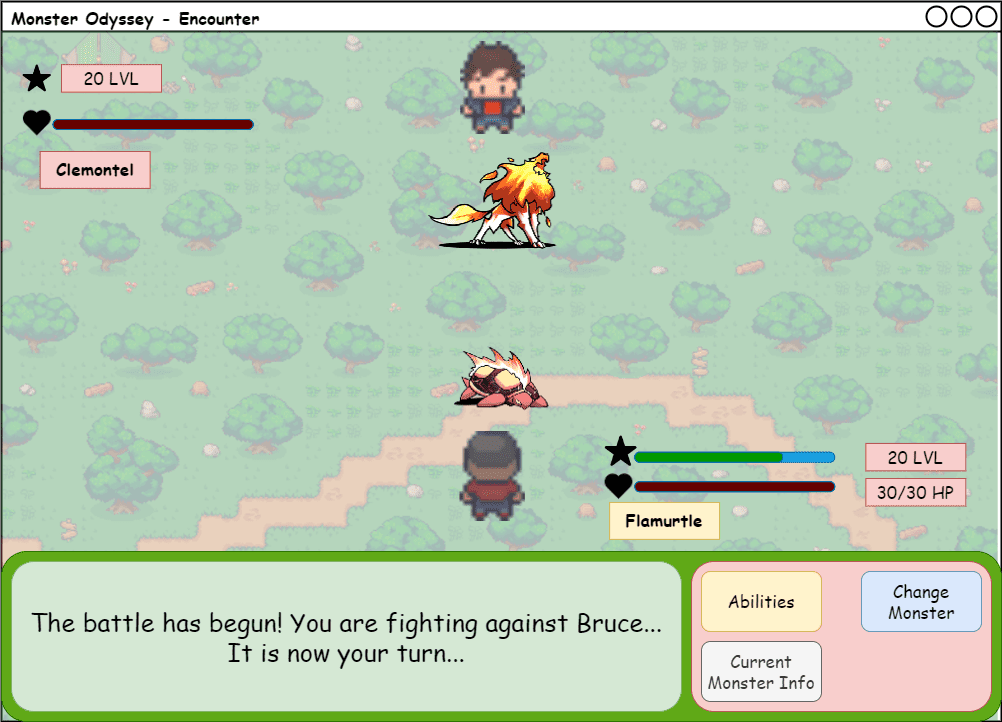
\includegraphics[width=\textwidth]{images/mockups/Encounter/Encounter1v1.png}
        \caption{Eins-gegen-Eins Kampfsituation Trainer}
        \label{fig: Eins-gegen-Eins Kampfsituation Trainer}
    \end{subfigure}
    \hfill
    \begin{subfigure}[b]{0.4\textwidth}
        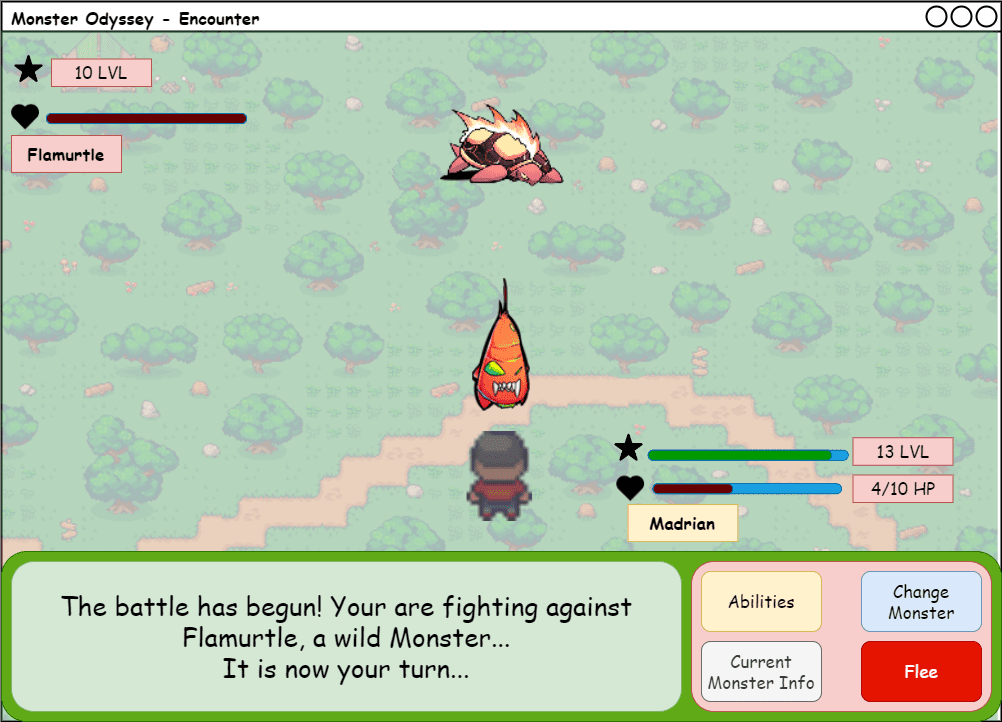
\includegraphics[width=\textwidth]{images/mockups/Encounter/EncounterWild.png}
        \caption{Eins-gegen-Eins Kampfsituation gegen wilden Monster}
        \label{fig: Eins-gegen-Eins Kampfsituation gegen wilden Monster}
    \end{subfigure}
    \caption{Mockup: Eins-gegen-Eins Kampfsituation}
    \label{fig: Eins-gegen-Eins Kampfsituation}
\end{figure}
\begin{figure}[H]
    \centering
    \begin{subfigure}[b]{0.4\textwidth}
        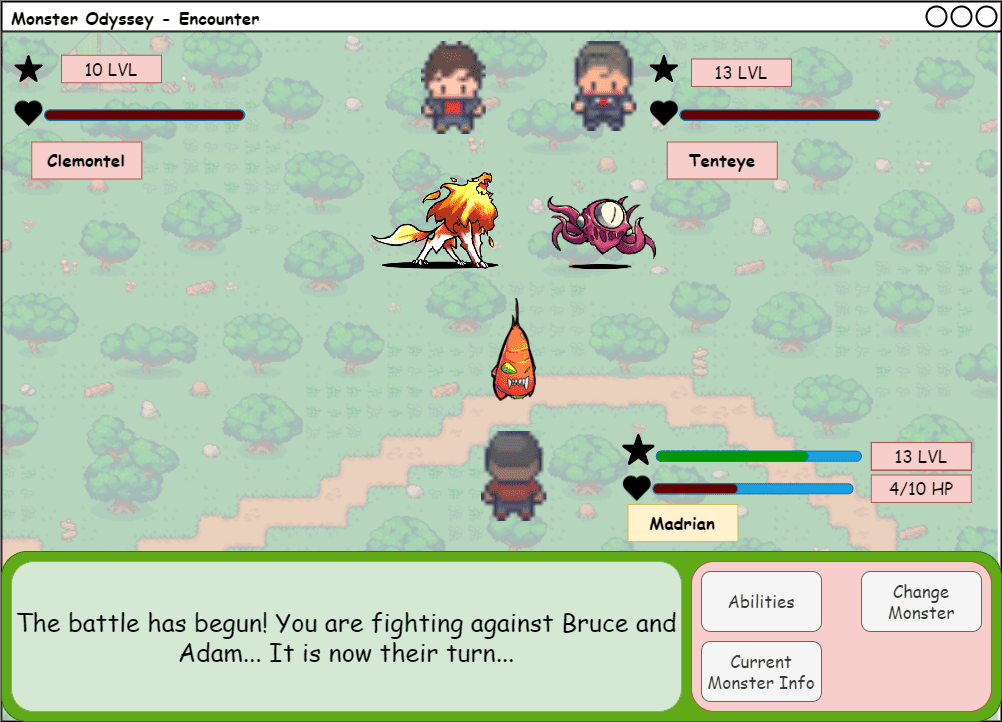
\includegraphics[width=\textwidth]{images/mockups/Encounter/Encounter1v2.png}
        \caption{Eins-gegen-Zwei Kampfsituation}
        \label{fig: Eins-gegen-Zwei Kampfsituation}
    \end{subfigure}
    \hfill
    \begin{subfigure}[b]{0.4\textwidth}
        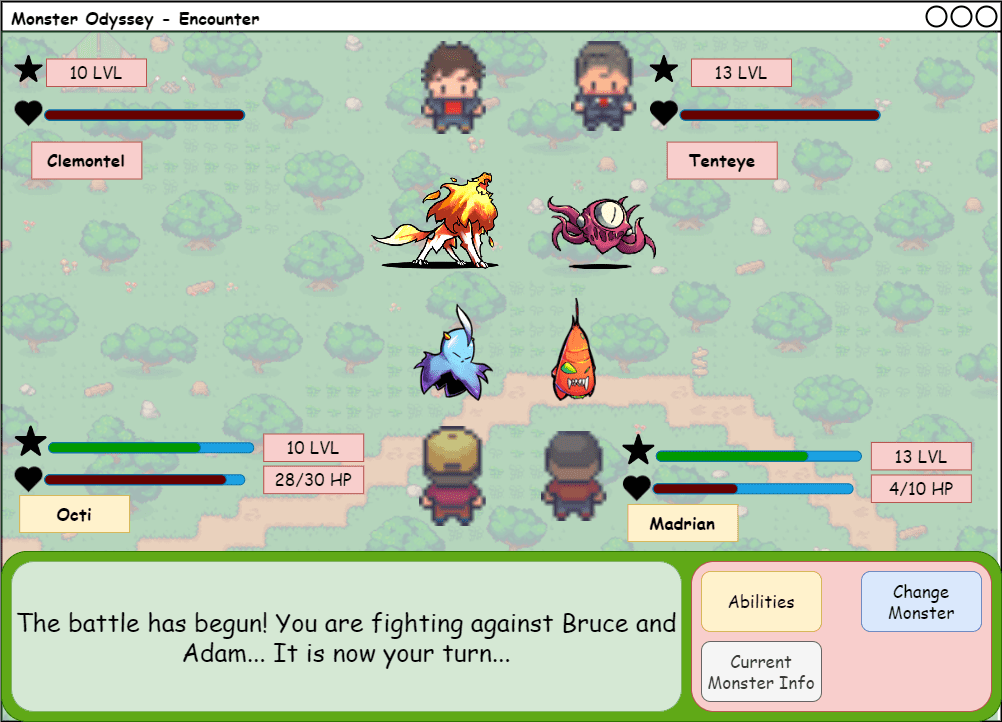
\includegraphics[width=\textwidth]{images/mockups/Encounter/Encounter2v2.png}
        \caption{Zwei-gegen-Zwei Kampfsituation}
        \label{fig: Zwei-gegen-Zwei Kampfsituation}
    \end{subfigure}
    \caption{Mockup: Eins-gegen-Zwei und Zwei-gegen-Zwei Kampfsituationen}
    \label{fig:Eins-gegen-Zwei und Zwei-gegen-Zwei Kampfsituationen}
\end{figure}
Neben dem Textfeld befinden sich mehrere Knöpfe, die für den Kampf essenziell sind. Die zwei Knöpfe 'Abilities' und 'Change Monster' sind unter Umständen deaktiviert und je nach Kontext werden sie wieder aktiviert und klickbar, wohingegen der Knopf 'Current Monster Info' jederzeit verfügbar ist.
Mit dem ersten Knopf 'Abilities' aus beispielsweise Abbildung~\ref{fig: Eins-gegen-Eins Kampfsituation Trainer} kann der Nutzer die Fähigkeiten des aktuellen Monsters sehen. 
Mit dem Drücken einer Fähigkeit wie in Abbildung~\ref{fig: Fähigkeiten des jetzigen Monsters} wird diese Fähigkeit für den Zug des Nutzers gesetzt und der Server entscheidet, wessen Fähigkeit von beiden Trainern ausgeführt und angewandt wird.
Wenn eine Fähigkeit angewandt wird, sieht der Nutzer eine Benachrichtigung wie in Abbildung~\ref{fig: Fähigkeit auf den gegnerischen Monster angewandt} in dem Textfeld, in der der Name der verwendeten Fähigkeit, der Name des angegriffenen Monsters und die Effektivität des Angriffs erwähnt sind.
Weiterhin werden alle Attribute, der vom Angriff betroffenen Monster, aktualisiert.
Der Nutzer muss mit der Nutzung der Fähigkeiten sparsam umgehen, da es für die jeweilige Fähigkeit eine begrenzte Anzahl an Nutzungen, wie in der Abbildung~\ref{fig: Fähigkeiten des jetzigen Monsters} zu sehen ist, gibt.
Die Anzahl an übrigen Nutzungen sieht der Nutzer unter dem Namen der Fähigkeit in dem Knopf.
Darüber hinaus kann der Nutzer zu der ursprünglichen Ansicht aus der Abbildung~\ref{fig: Eins-gegen-Eins Kampfsituation Trainer} zurückkehren, wenn er den Pfeilknopf drückt.
\begin{figure}[H]
    \center
    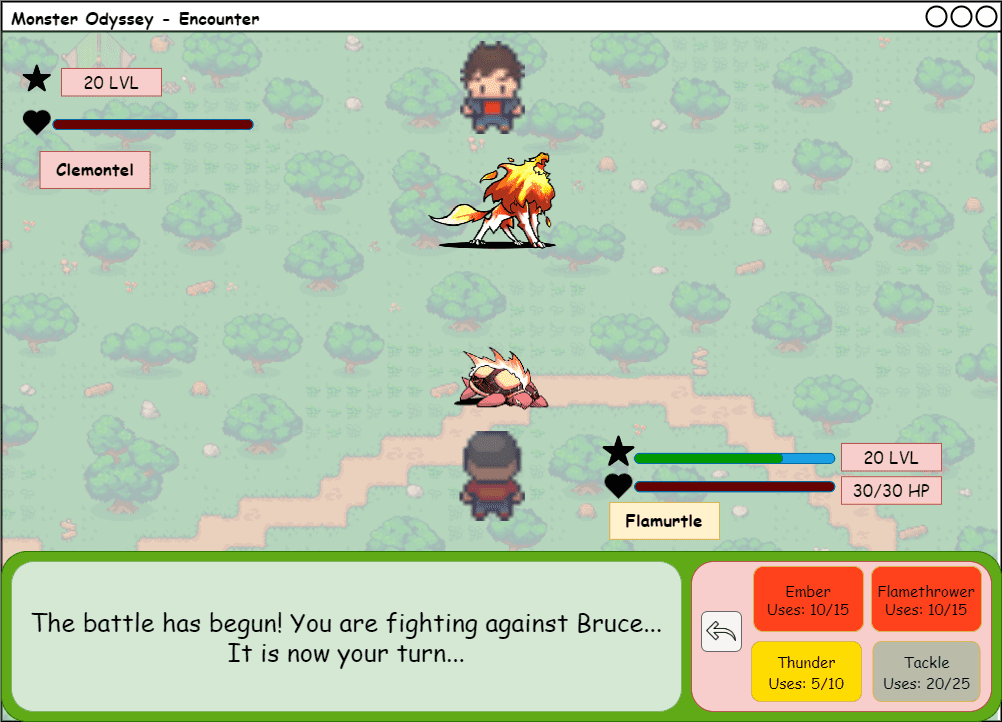
\includegraphics[scale=\scale]{images/mockups/Encounter/Encounter1v1Abilities.png}
    \caption{Mockup: Fähigkeiten des jetzigen Monsters}
    \label{fig: Fähigkeiten des jetzigen Monsters}
\end{figure}
\begin{figure}[H]
    \center
    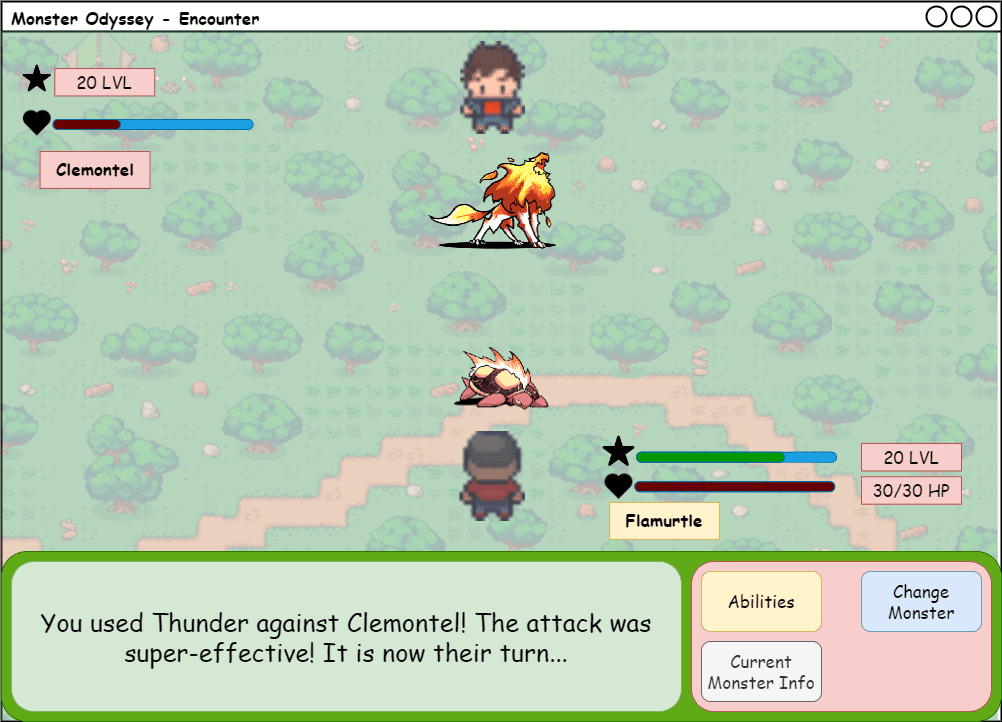
\includegraphics[scale=\scale]{images/mockups/Encounter/Encounter1v1AbilitiesUsed.png}
    \caption{Mockup: Fähigkeit auf das gegnerische Monster angewandt}
    \label{fig: Fähigkeit auf den gegnerischen Monster angewandt}
\end{figure}
Der Nutzer besiegt das gegnerische Monster, wenn seine Lebenspunkte auf null gesetzt sind.
Die Benachrichtigung in dem Textfeld wird entsprechend der Abbildung~\ref{fig: Gegnerischen Monster besiegt} angezeigt. 
Dabei erhält das jetzige Monster Erfahrungspunkte.
Sobald diese ausreichend für einen Levelaufstieg sind, bekommt der Monster neue persistente Attribute (Level, Schaden, max. Lebenspunkte, Geschwindigkeit und Verteidigung) und erlernt eine neue Fähigkeit, die in einem Fenster, wie in Abbildung~\ref{fig: Levelup mit neuen Werten und neuer Fähigkeit} zu sehen ist, dargestellt sind. 
Für die erlernte Fähigkeit werden der Name, eine kurze Beschreibung, die Stärke, die Präzision, die Anzahl der maximalen Nutzungen und der Typ der Fähigkeit angezeigt. 
Diese Fähigkeit wird nur dann erlernt, wenn das Monster weniger als vier Fähigkeiten besitzt.
Falls das Monster bereits vier Fähigkeiten aufweist, erscheint das Fenster ohne die erlernte Fähigkeit wie in Abbildung~\ref{fig: Levelup mit neuen Werten} aufgezeigt ist.

Sofern der Gegner keine anderen Monster mit Lebenspunkten \textgreater  0 hat, verliert der er den Kampf während der Nutzer den Kampf gewinnt. 
Es erscheint ein Popup, in welchem der Nutzer über den Gewinn, wie in der Abbildung~\ref{fig: Encounter gewonnen Ankündigung} gezeigt ist und über das Verlassen der Kampfszene beachrichtigt wird.
Die Kampfszene wird erst verlassen und zum Spielbildschirm gewechselt, sobald der Nutzer auf den 'OK'-Knopf aus der Abbildung~\ref{fig: Encounter gewonnen Ankündigung} gedrückt hat.
Falls der Gegner das aktuelle Monster des Nutzers, wie in Abbildung~\ref{fig: Jetziger Monster besiegt} dargestellt ist, besiegt und der Nutzer kein anderes Monster mit Lebenspunkten \textgreater  0 besitzt, erscheint ein Popup wie in Abbildung~\ref{fig: Encounter verloren Ankündigung} mit der gleichen Funktionalität wie das Popup aus Abbildung~\ref{fig: Encounter gewonnen Ankündigung}.
\begin{figure}[H]
    \center
    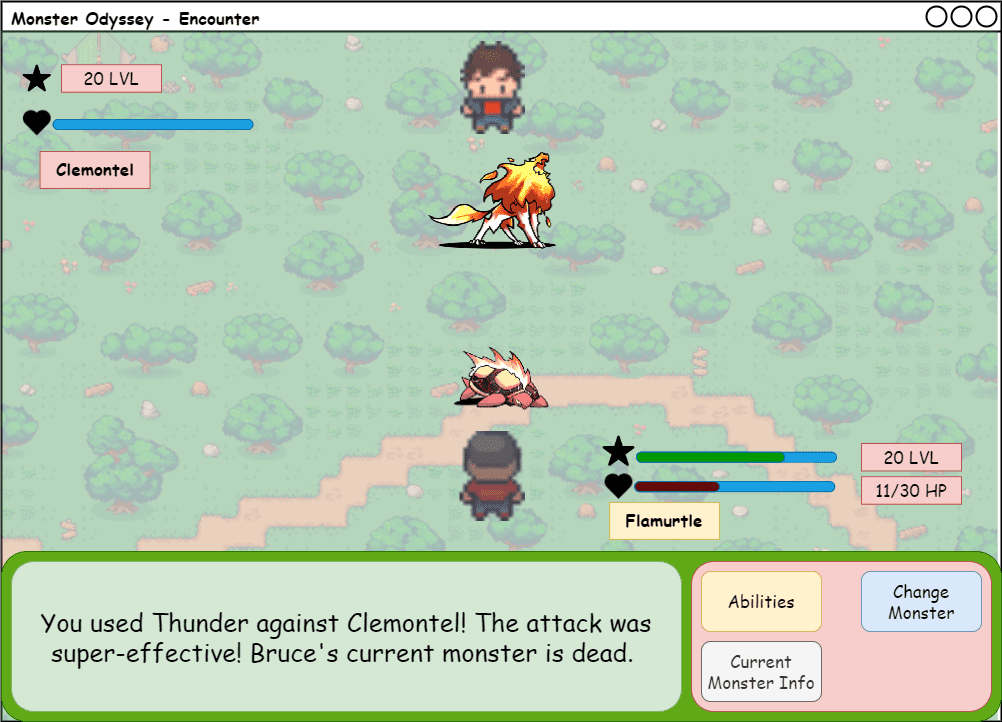
\includegraphics[scale=\scale]{images/mockups/Encounter/Encounter1v1AbilitiesUsedWon.png}
    \caption{Mockup: Gegnerischer Monster besiegt}
    \label{fig: Gegnerischen Monster besiegt}
\end{figure}
\begin{figure}[H]
    \center
    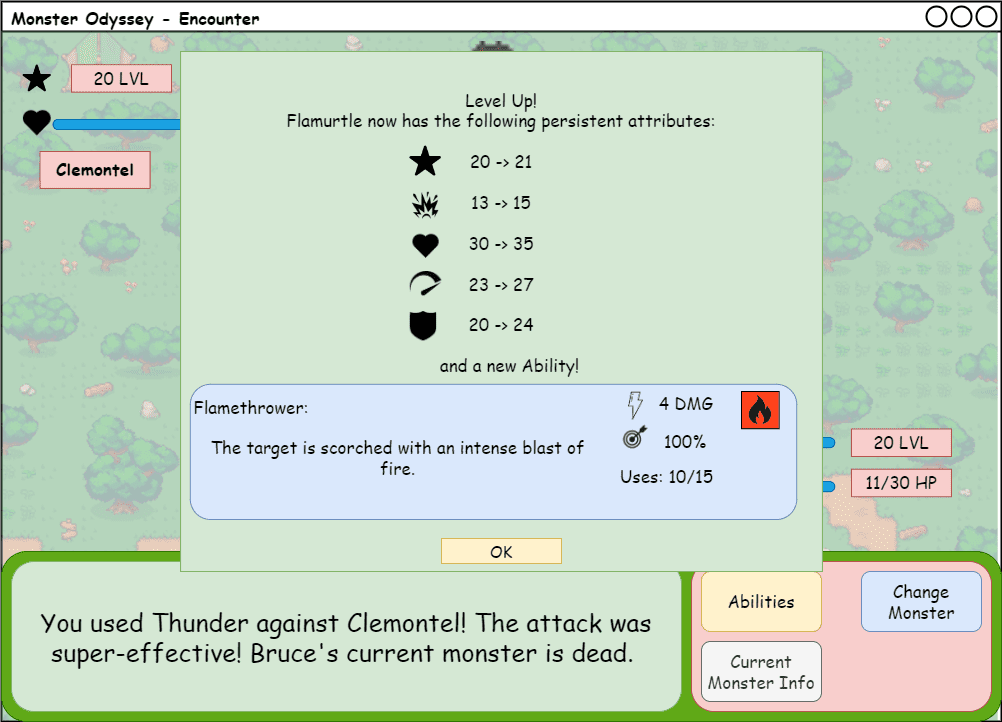
\includegraphics[scale=\scale]{images/mockups/Encounter/Encounter1v1AbilitiesUsedWonLevelUp.png}
    \caption{Mockup: Levelup mit neuen Werten und neuer Fähigkeit}
    \label{fig: Levelup mit neuen Werten und neuer Fähigkeit}
\end{figure}
\begin{figure}[H]
    \center
    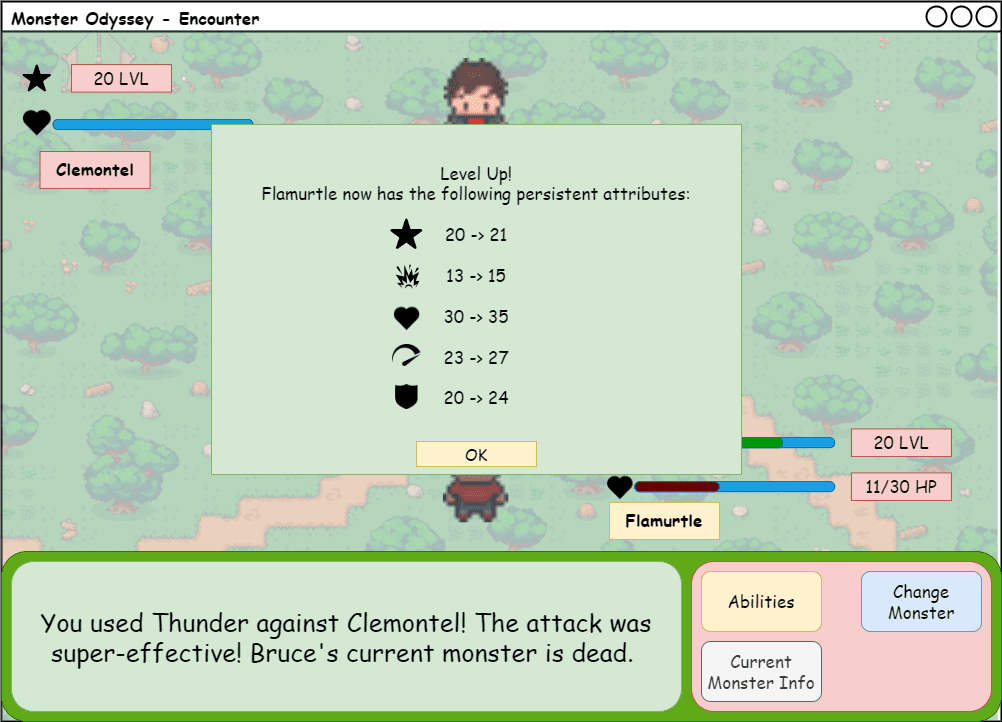
\includegraphics[scale=\scale]{images/mockups/Encounter/Encounter1v1AbilitiesUsedWonLevelUpNoAbility.png}
    \caption{Mockup: Levelup mit neuen Werten}
    \label{fig: Levelup mit neuen Werten}
\end{figure}
\begin{figure}[H]
    \center
    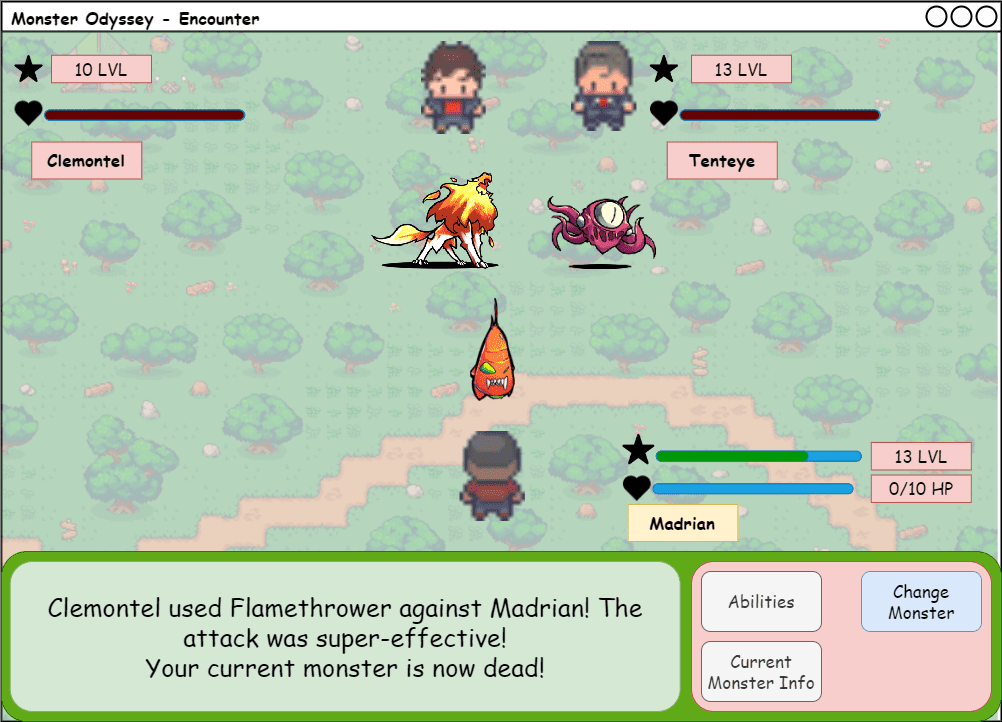
\includegraphics[scale=\scale]{images/mockups/Encounter/Encounter1v2OpponentAttackedAndLost.png}
    \caption{Mockup: Jetziger Monster besiegt}
    \label{fig: Jetziger Monster besiegt}
\end{figure}
\begin{figure}[H]
    \centering
    \begin{subfigure}[b]{0.4\textwidth}
        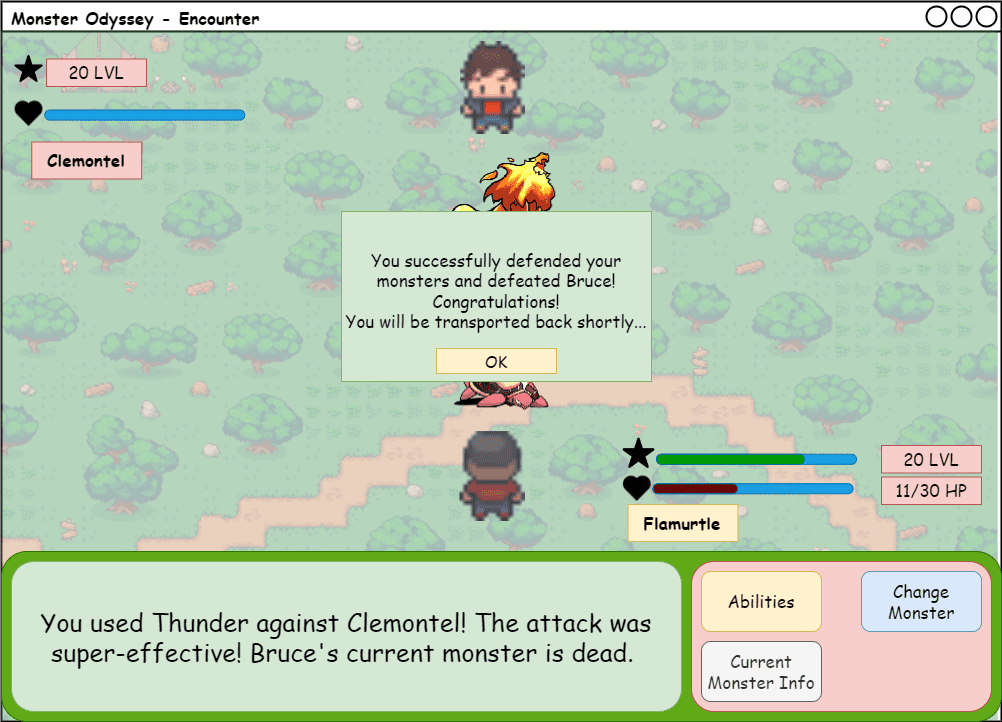
\includegraphics[width=\textwidth]{images/mockups/Encounter/Encounter1v1AbilitiesUsedWonGoBack.png}
        \caption{Kampf gewonnen}
        \label{fig: Encounter gewonnen Ankündigung}
    \end{subfigure}
    \hfill
    \begin{subfigure}[b]{0.4\textwidth}
        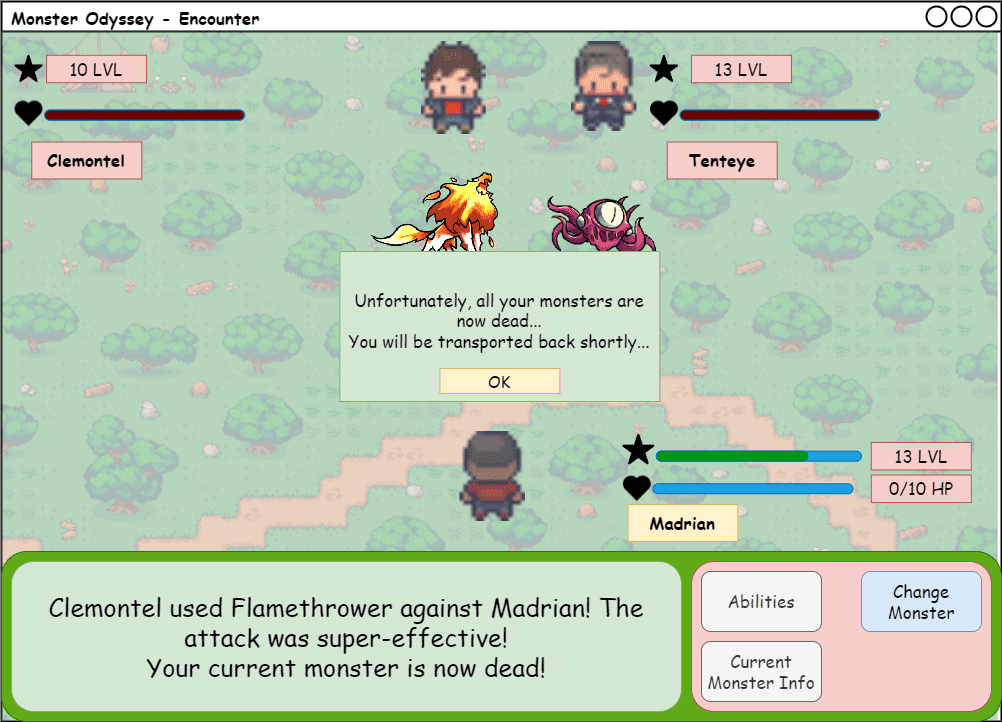
\includegraphics[width=\textwidth]{images/mockups/Encounter/Encounter1v2OpponentAttackedAndLostPopup.png}
        \caption{Kampf verloren}
        \label{fig: Encounter verloren Ankündigung}
    \end{subfigure}
    \caption{Mockup: Kampf beendet}
    \label{fig: Encounter beendet}
\end{figure}
Der Nutzer hat außerdem die Gelegenheit, Informationen über das aktuelle Monster aufzurufen. Dabei werden verschiedene Attribute für das Monster dargestellt, die für den Kampf eine hohe Relevanz aufweisen. Das Informationsfenster erscheint, wenn der Nutzer den Knopf 'Current Monster Info' aus Abbildung~\ref{fig: Informationen über den jetzigen Monster} drückt. In dem Fenster aus Abbildung~\ref{fig: Informationen über den jetzigen Monster} kann der Nutzer das Bild, die persistenten und aktuellen Attribute als Balken und Zahl, den Typen und die Fähigkeiten des Monsters sehen. Für die jeweilige Fähigkeit ist eine Übersicht, wie in Abbildung~\ref{fig: Levelup mit neuen Werten und neuer Fähigkeit} gezeigt ist, für die erlernte Fähigkeit vorhanden.  
\begin{figure}[H]
    \center
    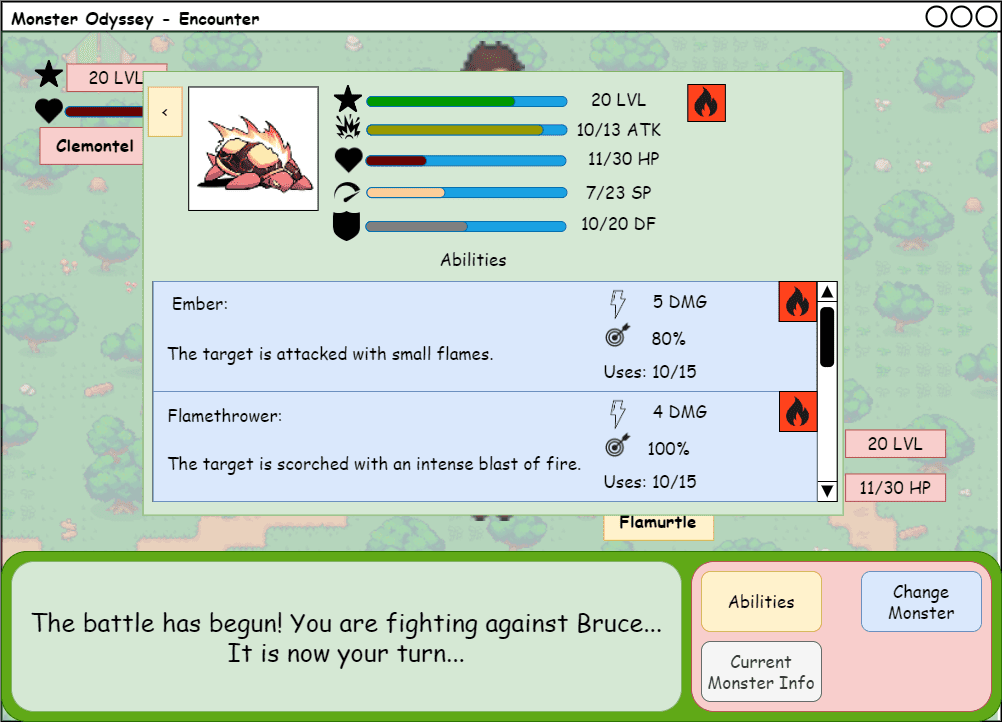
\includegraphics[scale=\scale]{images/mockups/Encounter/Encounter1v1Info.png}
    \caption{Mockup: Informationen über den jetzigen Monster}
    \label{fig: Informationen über den jetzigen Monster}
\end{figure}
Befindet sich der Nutzer in einer Eins-gegen-Zwei oder Zwei-gegen-Zwei Kampfsituation und der Nutzer möchte eine Fähigkeit anwenden, dann muss der Nutzer das Ziel auswählen, mit welchem gegnerische Monster angegriffen werden sollen. 
Dem Nutzer wird wie in Abbildung~\ref{fig: Ziel auswählen} ein Hinweis gegeben. Der Nutzer wird aufgefordert auf das gewünschte gegnerische Monster zu klicken, um das Ziel auszuwählen. 
\begin{figure}[H]
    \center
    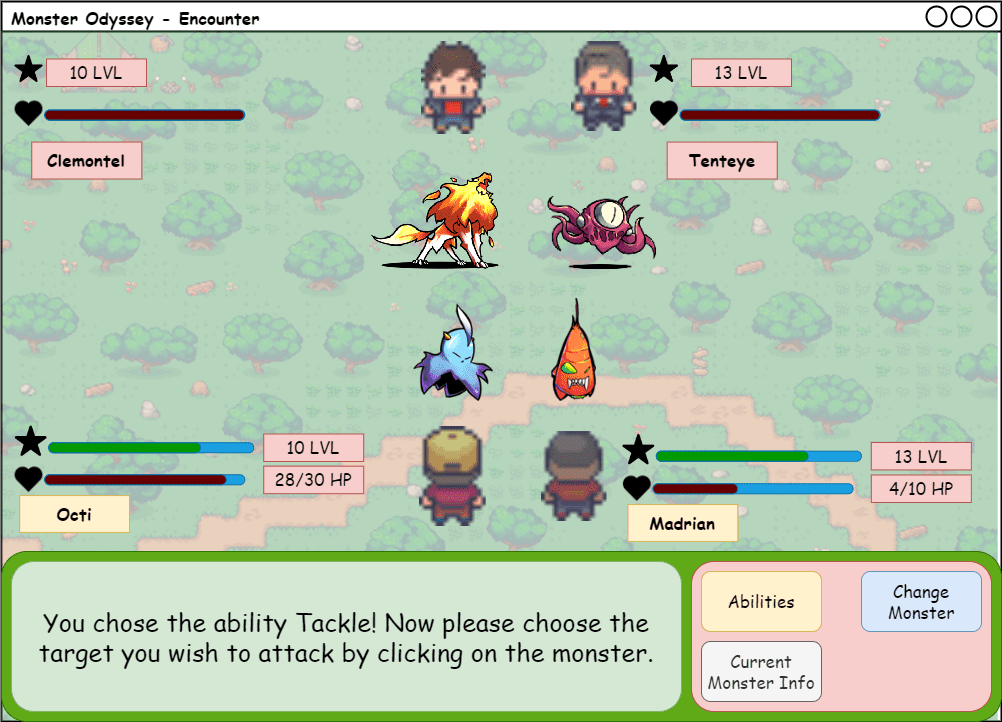
\includegraphics[scale=\scale]{images/mockups/Encounter/Encounter2v2ChooseTarget.png}
    \caption{Mockup: Ziel auswählen}
    \label{fig: Ziel auswählen}
\end{figure}
Es können Kampfsituationen auftreten, in denen das jetzige Monster schwächer als das gegnerische Monster wird. 
In diesem Fall hat der Nutzer die Möglichkeit das jetzige Monster gegen ein stärkeres Monster aus seinem Team auszuwechseln, indem der Nutzer auf den 'Change Monster'-Knopf aus Abbildung~\ref{fig: Monster wechseln Popup} drückt. 
Damit öffnet sich ein Fenster wie in Abbildung~\ref{fig: Monster wechseln Popup}, in welchem die verfügbaren Monster aus dem Team des Nutzers aufgelistet sind. Für jedes Monster auf der Liste gibt es zwei Knöpfe: einen Knopf für die Monsterinformationen und einen Knopf zum Wechseln des aktiven Monsters. 
Nach der Auswahl eines neuen aktiven Monster erscheint dieses Monster wie in Abbildung~\ref{fig: Monster ausgewechselt} vor der Trainerfigur des Nutzers und alle Attribute werden entsprechend aktualisiert.
Außerdem wird der Nutzer in dem Protokoll auf das Ereignis hingewiesen. 
\begin{figure}[H]
    \centering
    \begin{subfigure}[b]{0.4\textwidth}
        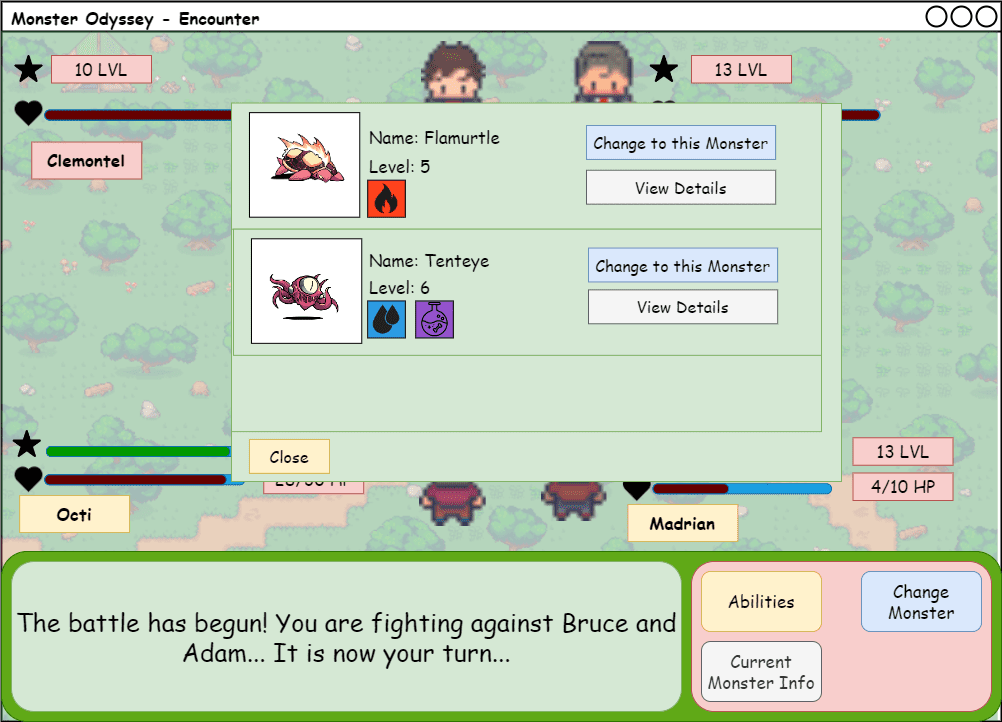
\includegraphics[width=\textwidth]{images/mockups/Encounter/Encounter2v2ChangeMonsterPopup.png}
        \caption{Monster auswechseln Popup}
        \label{fig: Monster wechseln Popup}
    \end{subfigure}
    \hfill
    \begin{subfigure}[b]{0.4\textwidth}
        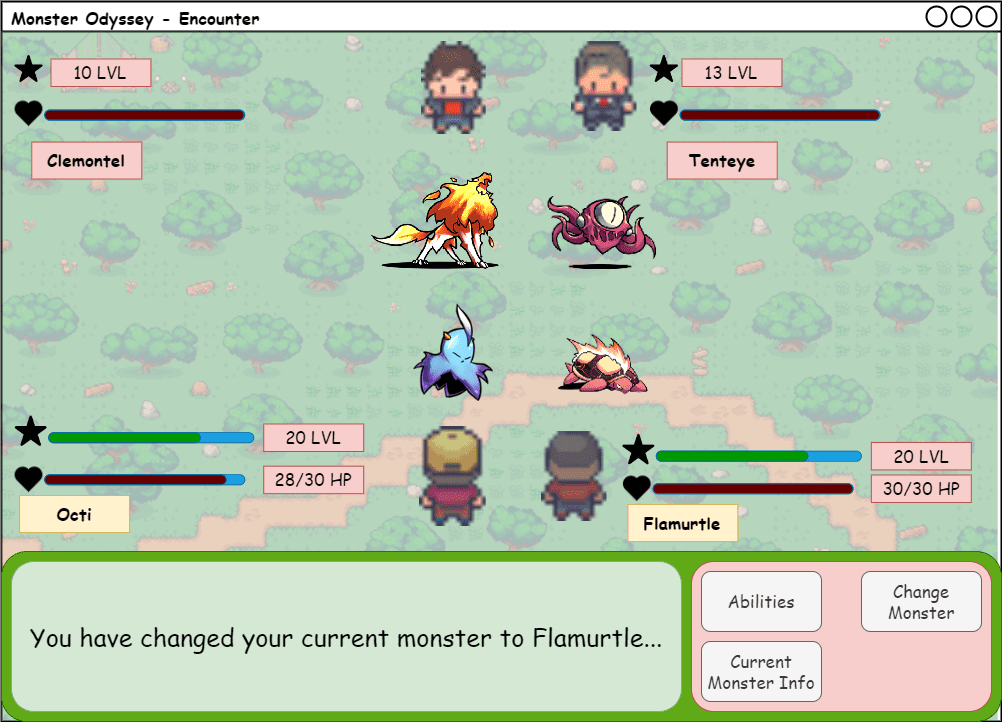
\includegraphics[width=\textwidth]{images/mockups/Encounter/Encounter2v2ChangeMonster.png}
        \caption{Monster ausgewechselt}
        \label{fig: Monster ausgewechselt}
    \end{subfigure}
    \caption{Mockup: Monster auswechseln}
    \label{fig: Monster auswechseln}
\end{figure}
Begegnet der Nutzer einem wilden Monster in hohem Gras und möchte gegen dieses Monster nicht kämpfen, dann kann der Nutzer aus dem Kampf fliehen, was bei den restlichen Kampfsituationen nicht möglich ist.
Der Nutzer kann aus dem Kampf beim Drücken auf den 'Flee'-Knopf aus der Abbildung~\ref{fig: Von wildem Monster fliehen Popup} fliehen. Somit wird ein Popup, wie in Abbildung~\ref{fig: Von wildem Monster fliehen Popup} angezeigt, in dem die Bestätigung des Nutzers für die Aktion benötigt wird.
Beim Drücken auf 'No' wird der Kampf fortgesetzt und beim Drücken auf 'Yes' wird das Fliehen bestätigt.
Anschließend wird der Nutzer in dem Ereignisprotokoll wie in Abbildung~\ref{fig: Von wildem Monster geflohen} darauf hingewiesen, dass der Nutzer aus der Kampfszene geflohen ist und die Szene in Kürze zum Spielbildschirm gewechselt wird. Das Wechseln der Szene erfolgt dann wenige Sekunden nach der Bekanntgabe. 
\begin{figure}[H]
    \centering
    \begin{subfigure}[b]{0.4\textwidth}
        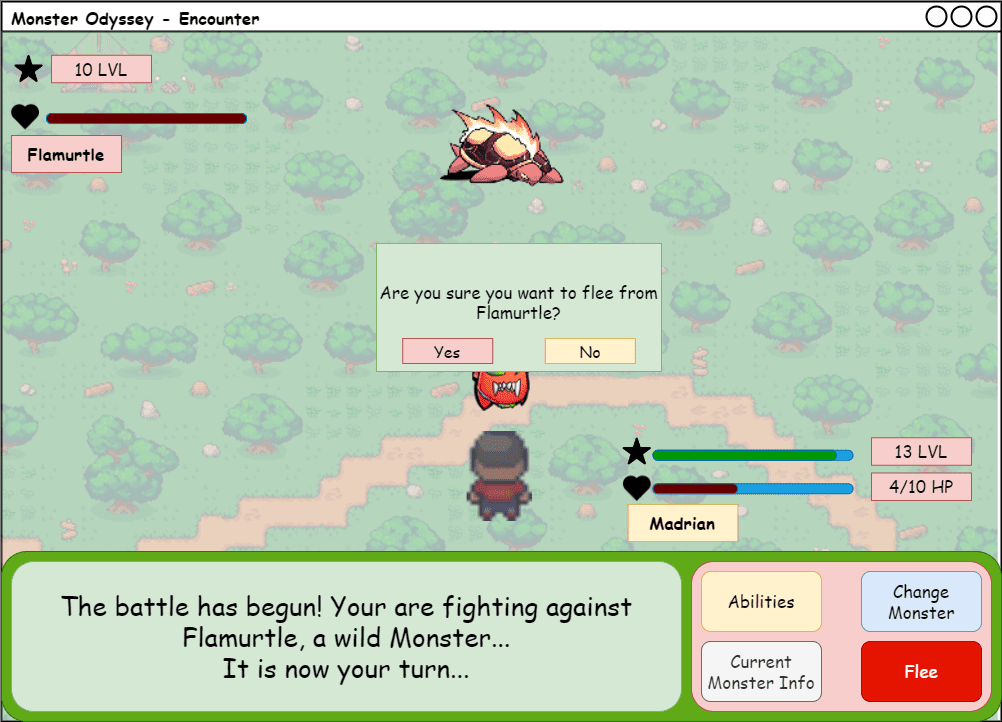
\includegraphics[width=\textwidth]{images/mockups/Encounter/EncounterWildFleePopUp.png}
        \caption{Popup beim Fliehen}
        \label{fig: Von wildem Monster fliehen Popup}
    \end{subfigure}
    \hfill
    \begin{subfigure}[b]{0.4\textwidth}
        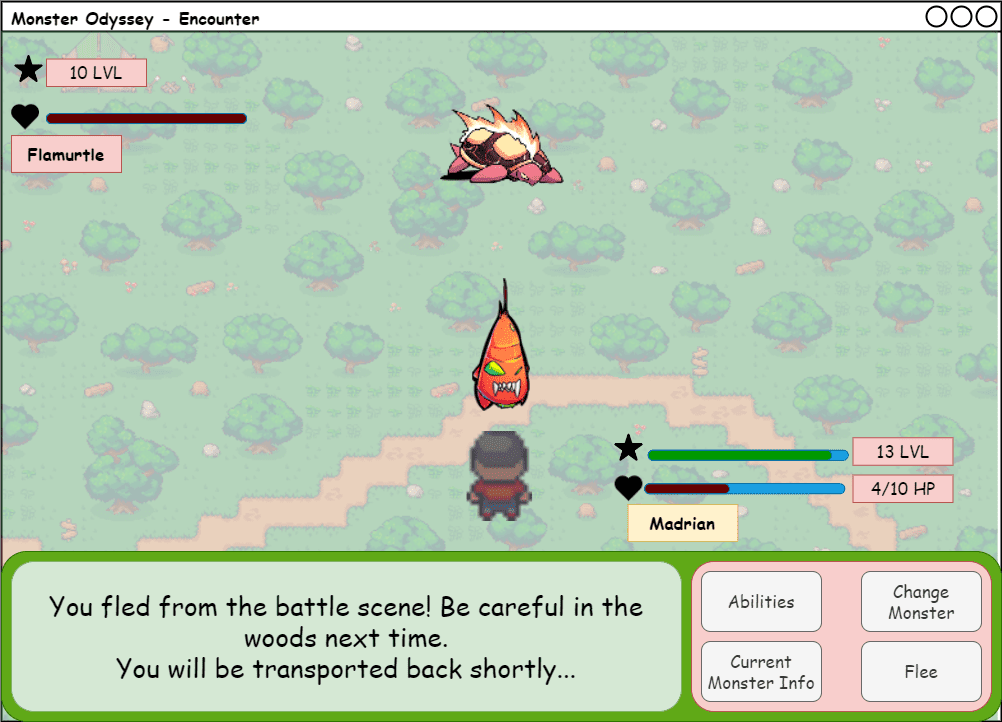
\includegraphics[width=\textwidth]{images/mockups/Encounter/EncounterWildFleed.png}
        \caption{Von wildem Monster geflohen}
        \label{fig: Von wildem Monster geflohen}
    \end{subfigure}
    \caption{Mockup: Fliehen von einem wilden Monster}
    \label{fig: Fliehen von einem wilden Monster}
\end{figure}

\subsection{Vergleich zwischen Mockups und Implementierung}\label{subsec:vergleich-zwischen-mockups-und-implementierung-kampf-führen}
Es bestehen viele Unterschiede zwischen den Mockups und der Implementierung, die auf der Ästhetik beziehungsweise der besseren Handhabung basieren. Im Folgenden werden die Unterschiede anhand der Szenarien Eins-gegen-Eins gegen einen Trainer und ein wildes Monster verdeutlicht. In der Abbildung~\ref{fig: Vergleich: Eins-gegen-Eins Kampfsituation Trainer} sind verschiedene Unterschiede anzumerken. Die Symbole für die Attribute 'Level' und 'Lebenspunkte' sind für die Übersichtlichkeit mit einer entsprechenden Farbe gekennzeichnet.
Der Namensbehälter von den Monstern ist etwas größer gestaltet, da es Monster mit längeren Namen gibt, die entsprechend mehr Platz benötigen.
Außerdem ist die Position des gegnerischen Trainers nach rechts verschoben. Der Grund der Verschiebung beruht auf der dynamischen Anzahl der gegnerischen Trainer, damit das Betreten eines neuen Trainers in den Kampf erleichtert wird.
Darüber hinaus sind die Balken größer und mit weißem Hintergrund ausgestattet. Das genaue Design aus den Mockups konnte wegen des Schwierigkeitsgrads nicht erzielt werden, wobei der weiße Hintergrund für eine klare Trennung zwischen dem maximalen Wert und dem tatsächlichem Wert sorgt.
Zudem ist die Darstellung der Lebenspunkte der Monster, die von dem Server vorgegebenen sind, mit einer Kommazahl anstatt einer ganzen Zahl ausgestattet.
In dem Ereignisprotokoll ist der letzte Satz weggelassen worden, da die Züge nicht nacheinander stattfinden, sondern beide Trainer ihren Zug gleichzeitig tätigen. Dabei ist der Text für das Ereignisprotokoll in fettgedruckter Schreibweise formuliert, was für den Nutzer eine bessere Lesbarkeit gewährleistet.
\begin{figure}[H]
    \centering
    \begin{subfigure}[b]{0.4\textwidth}
        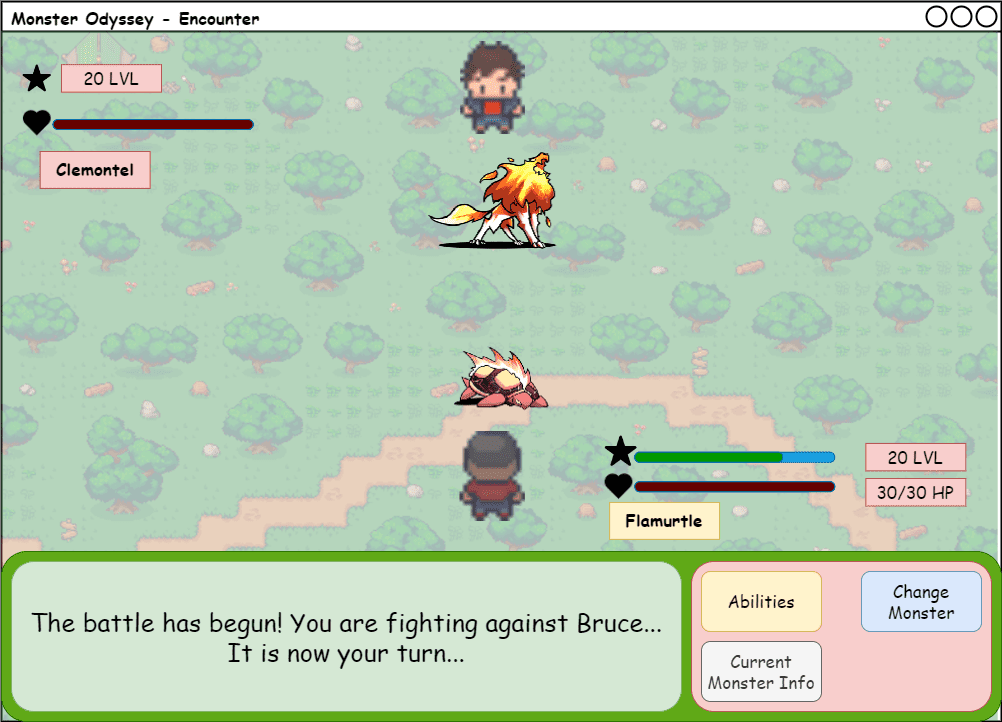
\includegraphics[width=\textwidth]{images/mockups/Encounter/Encounter1v1.png}
        \caption{Mockup:\phantom{EinsEins} Eins-gegen-Eins Kampfsituation Trainer}
        \label{fig: Mockup: Eins-gegen-Eins Kampfsituation Trainer}
    \end{subfigure}
    \hfill
    \begin{subfigure}[b]{0.4\textwidth}
        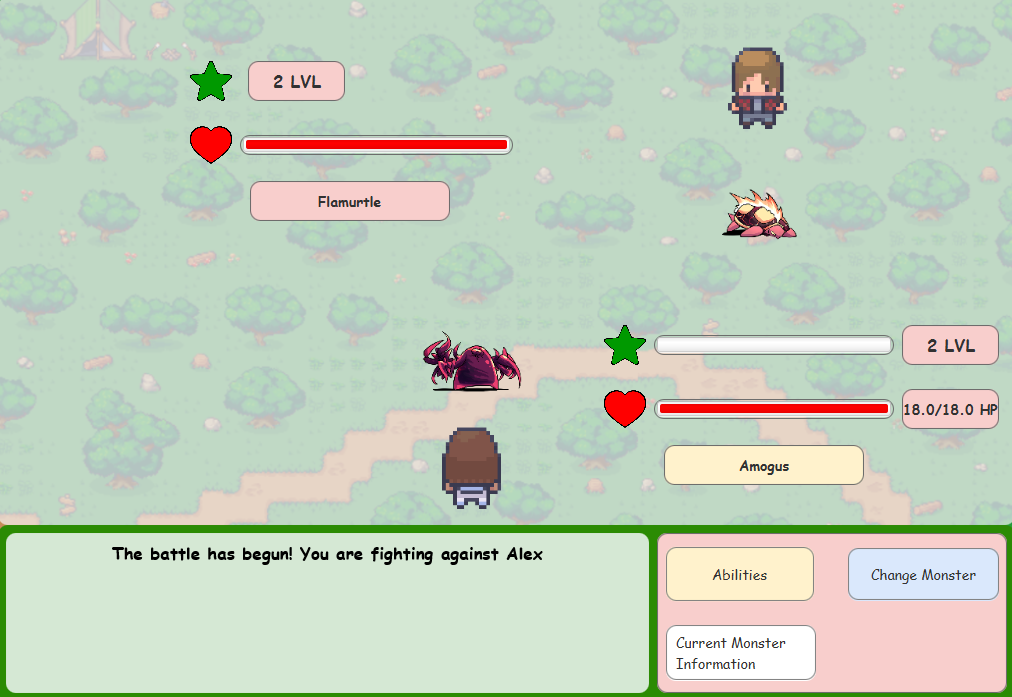
\includegraphics[width=\textwidth]{images/implementation/Encounter/1v1TrainervsTrainer.PNG}
        \caption{Implementierung: Eins-gegen-Eins Kampfsituation Trainer}
        \label{fig: Implementierung: Eins-gegen-Eins Kampfsituation Trainer}
    \end{subfigure}
    \caption{Vergleich: Eins-gegen-Eins Kampfsituation Trainer}
    \label{fig: Vergleich: Eins-gegen-Eins Kampfsituation Trainer}
\end{figure}
In der Abbildung~\ref{fig: Vergleich: Fähigkeiten des jetzigen Monsters} besteht ein Unterschied in der Darstellung der Fähigkeiten. Die Container der Fähigkeiten haben keine abgerundete Ecken. Der Unterschied dient nur der Ästhetik.

Beim Anwenden einer Fähigkeit wird das Ereignisprotokoll von dem Mockup verschieden dargestellt. Dabei wird der Text wie in der Abbildung~\ref{fig: Vergleich: Fähigkeit auf das gegnerische Monster angewandt} für die angewandte Fähigkeit des Gegners und des Trainers des Nutzers entsprechend aktualisiert. Das liegt daran, dass beide Parteien den Zug machen und somit das Ergebnis beider Fähigkeiten angezeigt werden muss. 
\begin{figure}[H]
    \centering
    \begin{subfigure}[b]{0.4\textwidth}
        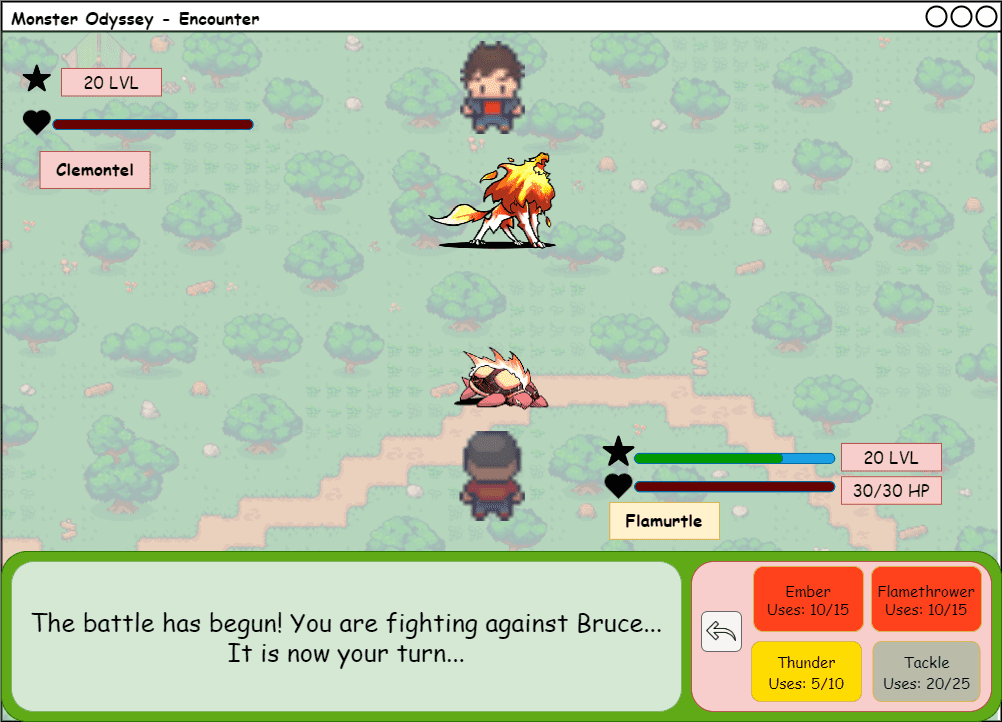
\includegraphics[width=\textwidth]{images/mockups/Encounter/Encounter1v1Abilities.png}
        \caption{Mockup: \phantom{desdes jetz}Fähigkeiten des jetzigen Monsters}
        \label{fig: Mockup: Fähigkeiten des jetzigen Monsters}
    \end{subfigure}
    \hfill
    \begin{subfigure}[b]{0.4\textwidth}
        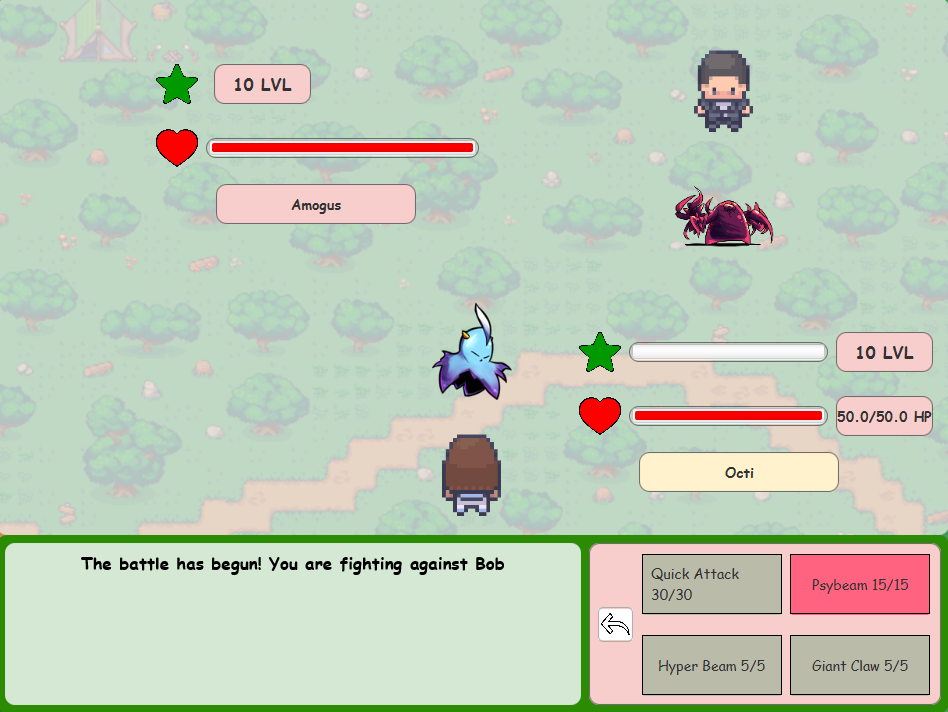
\includegraphics[width=\textwidth]{images/implementation/Encounter/abilities.PNG}
        \caption{Implementierung: Fähigkeiten des jetzigen Monsters}
        \label{fig: Implementierung: Fähigkeiten des jetzigen Monsters}
    \end{subfigure}
    \caption{Vergleich: Fähigkeiten des jetzigen Monsters}
    \label{fig: Vergleich: Fähigkeiten des jetzigen Monsters}
\end{figure}
\begin{figure}[H]
    \centering
    \begin{subfigure}[b]{0.4\textwidth}
        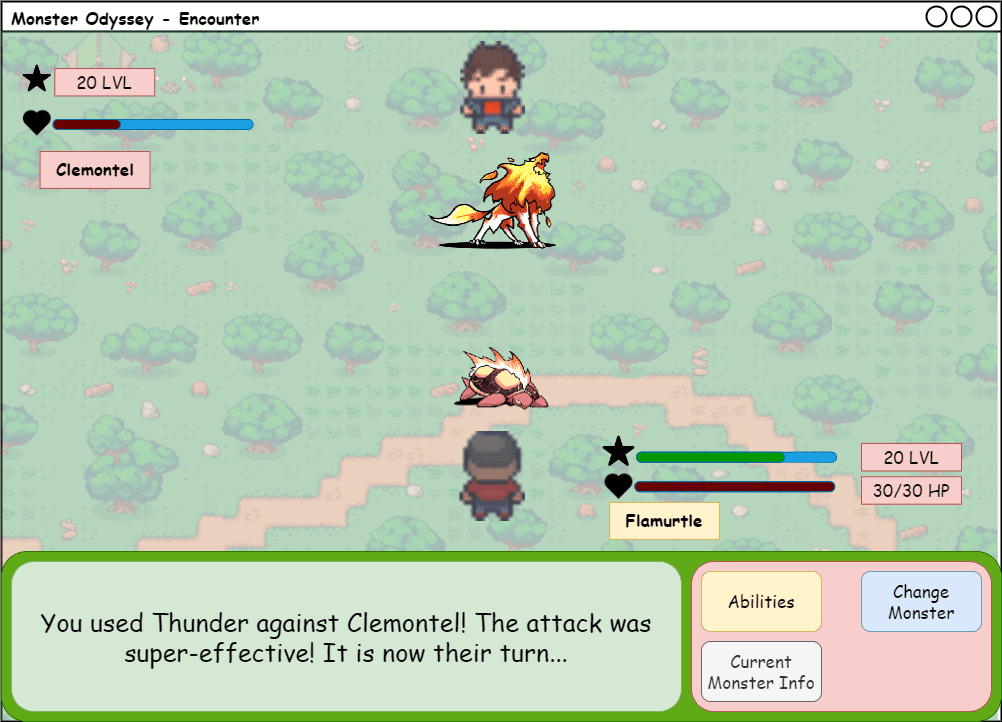
\includegraphics[width=\textwidth]{images/mockups/Encounter/Encounter1v1AbilitiesUsed.png}
        \caption{Mockup: \phantom{gewandt} Fähigkeit angewandt}
        \label{fig: Mockup: Fähigkeit auf das gegnerische Monster angewandt}
    \end{subfigure}
    \hfill
    \begin{subfigure}[b]{0.4\textwidth}
        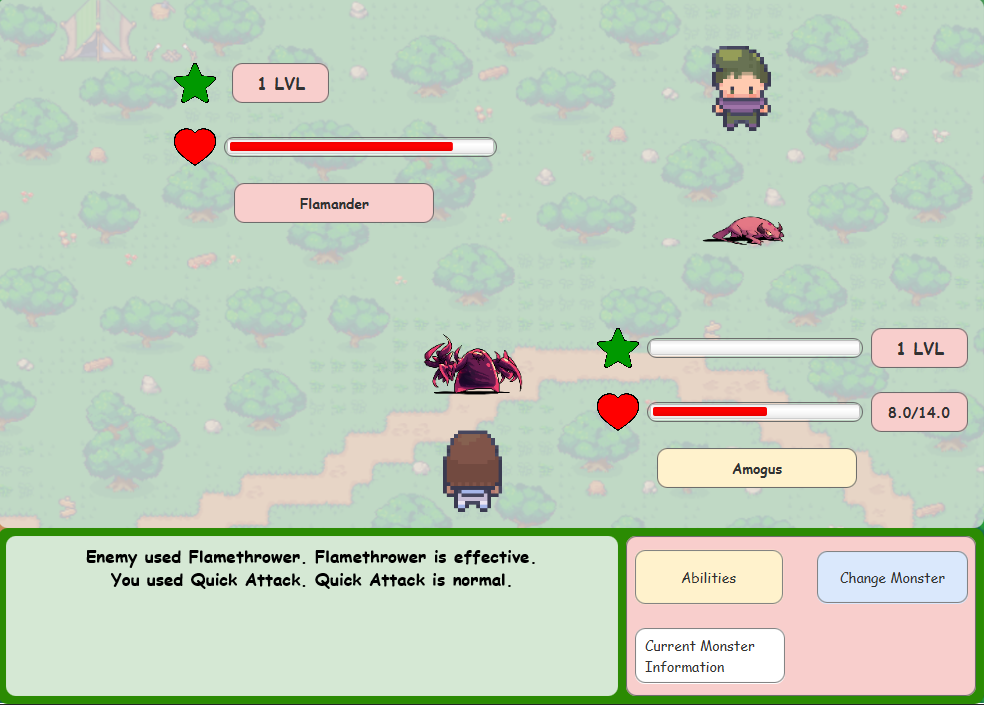
\includegraphics[width=\textwidth]{images/implementation/Encounter/abilitiesused.PNG}
        \caption{Implementierung: Fähigkeit angewandt}
        \label{fig: Implementierung: Fähigkeit auf das gegnerische Monster angewandt}
    \end{subfigure}
    \caption{Vergleich: Fähigkeit angewandt}
    \label{fig: Vergleich: Fähigkeit auf das gegnerische Monster angewandt}
\end{figure}
Zwischen den Mockups und der Implementierung beim Verlust oder Gewinn eines Kampfs bestehen zwei Unterschiede, die aufgrund von fehlender Qualitätssicherung wegen Zeitproblemen vor dem Releaseende enstanden sind. Zum einen wird das Fenster wie in der Abbildung~\ref{fig: Vergleich: Kampf verloren} größer als nötig dargestellt und zum anderen spiegelt sich der aktuelle Status des Kampfs nicht in dem Ereignisprotokoll wider.

In der Abbildung~\ref{fig: Vergleich: Levelup mit neuen Werten und neuer Fähigkeit} besteht bezüglich des Levelaufstiegs des eigenen Monsters ein Unterschied bei der Reihenfolge der geänderten Attribute. Die Reihenfolge ist dennoch für den Nutzer nicht ausschlaggebend und weist keine Funktionalitätsänderung auf. Darüber hinaus konnte die erworbene Fähigkeit nicht in dem designierten Bereich dargestellt werden, da es Zeitprobleme vor dem Releaseende beim Abschließen der entsprechenden User Story gegeben hat.
\begin{figure}[H]
    \centering
    \begin{subfigure}[b]{0.4\textwidth}
        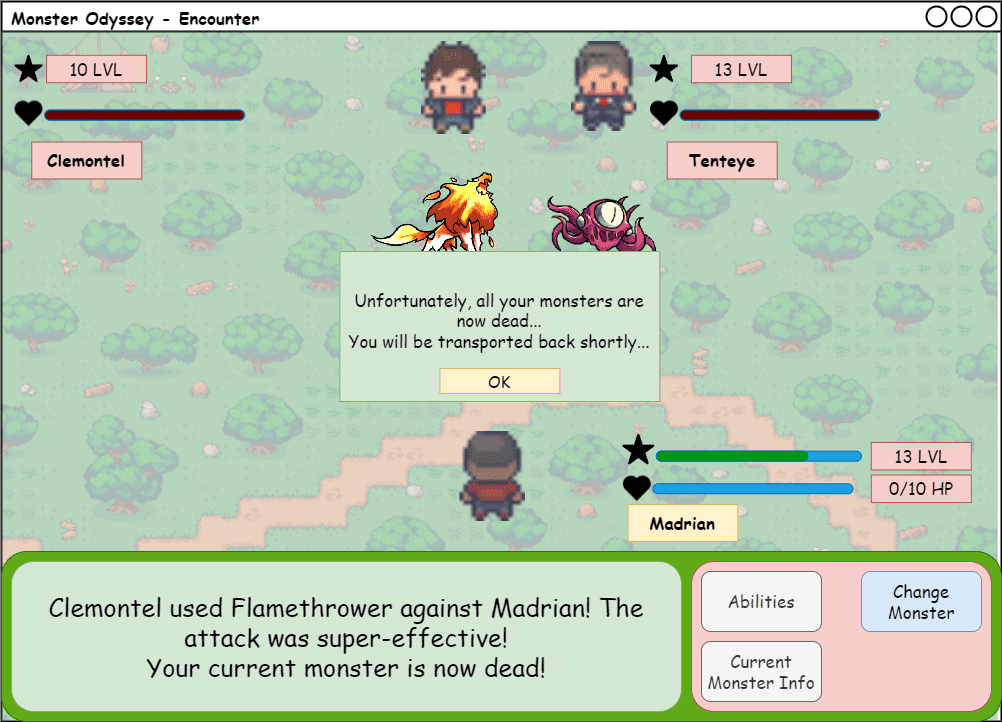
\includegraphics[width=\textwidth]{images/mockups/Encounter/Encounter1v2OpponentAttackedAndLostPopup.png}
        \caption{Mockup: \phantom{Kampfve}Kampf verloren}
        \label{fig: Mockup: Kampf verloren}
    \end{subfigure}
    \hfill
    \begin{subfigure}[b]{0.4\textwidth}
        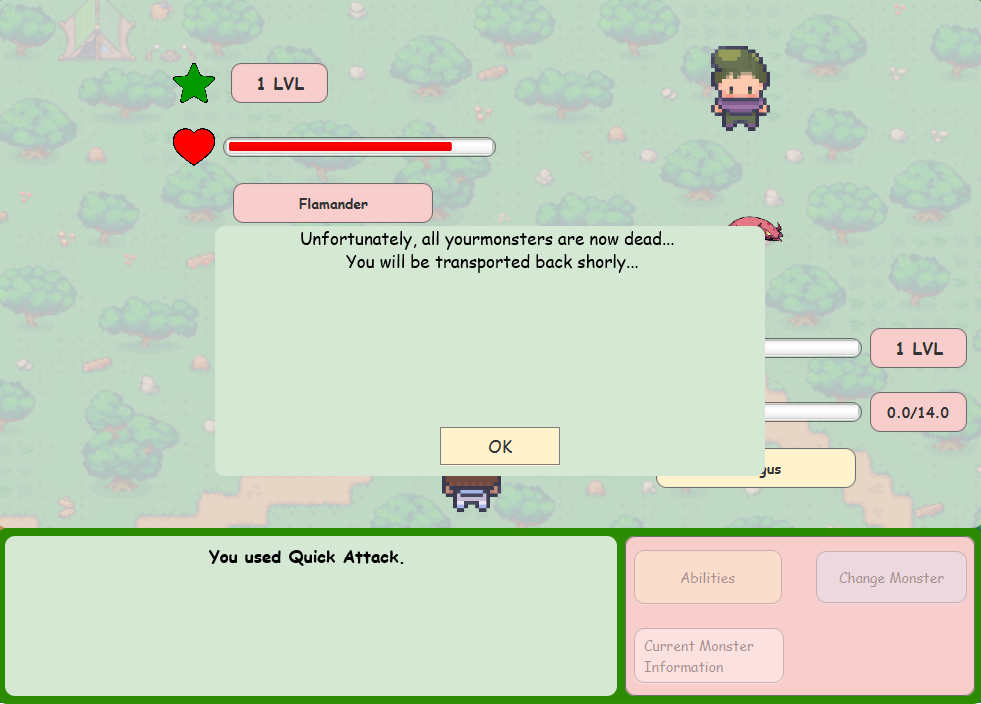
\includegraphics[width=\textwidth]{images/implementation/Encounter/encounterverloren.PNG}
        \caption{Implementierung: Kampf verloren}
        \label{fig: Implementierung: Kampf verloren}
    \end{subfigure}
    \caption{Vergleich: Kampf verloren}
    \label{fig: Vergleich: Kampf verloren}
\end{figure}
\begin{figure}[H]
    \centering
    \begin{subfigure}[b]{0.4\textwidth}
        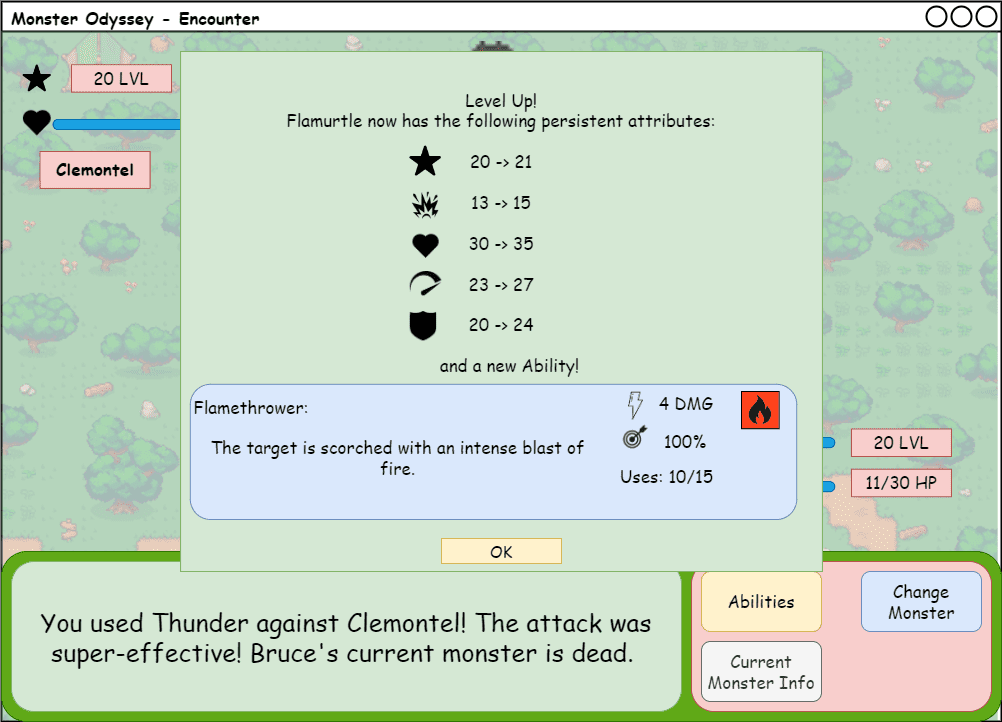
\includegraphics[width=\textwidth]{images/mockups/Encounter/Encounter1v1AbilitiesUsedWonLevelUp.png}
        \caption{Mockup: Levelup}
        \label{fig: Mockup: Levelup mit neuen Werten und neuer Fähigkeit}
    \end{subfigure}
    \hfill
    \begin{subfigure}[b]{0.4\textwidth}
        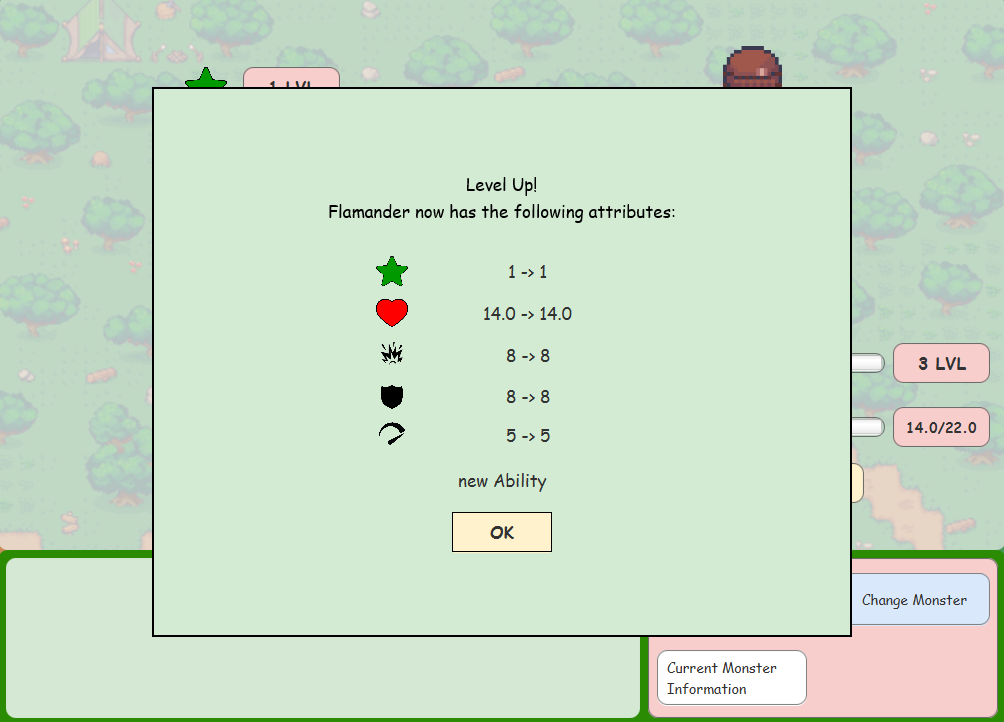
\includegraphics[width=\textwidth]{images/implementation/Encounter/Levelupmitneuerability.PNG}
        \caption{Implementierung: Levelup}
        \label{fig: Implementierung: Levelup mit neuen Werten und neuer Fähigkeit}
    \end{subfigure}
    \caption{Vergleich: Levelup mit neuen Werten und neuer Fähigkeit}
    \label{fig: Vergleich: Levelup mit neuen Werten und neuer Fähigkeit}
\end{figure}
Bei dem Monsterwechsel-Fenster sind wie in der Abbildung~\ref{fig: Vergleich: Monster auswechseln Popup} zwei Unterschiede anzumerken. Hinter dem jeweiligen Monsterbild wird kein weißer Hintergrund dargestellt und die Bezeichnung für den Wechselknopf ist leicht unterschiedlich. Die Unterschiede dienen allerdings nur der Ästhetik und haben keinen Einfluss auf die Funktionalität.

In der Abbildung~\ref{fig: Vergleich: Popup beim Fliehen} ist das Popup für das Fliehen etwas größer als nötig gestaltet, wobei auch der Text für die Bestätigung anders als der Text im Mockup ist. Jedoch wird dabei die Semantik des Fliehens immer noch beibehalten. Die Änderungen betreffen die Funktionalität nicht.

Nach der Bestätigung des Fliehens wird der Text aus dem Ereignisprotokoll wie in der Abbildung~\ref{fig: Vergleich: Von wildem Monster geflohen} nicht identisch dargestellt. Das liegt daran, dass hierbei auch keine Qualitätssicherung aufgrund von fehlender Zeit vor dem Releaseende durchgeführt werden konnte. Darüber hinaus wird beim Fliehen eine flüssige Animation angezeigt, um das Fliehen zu visualisieren.
\begin{figure}[H]
    \centering
    \begin{subfigure}[b]{0.4\textwidth}
        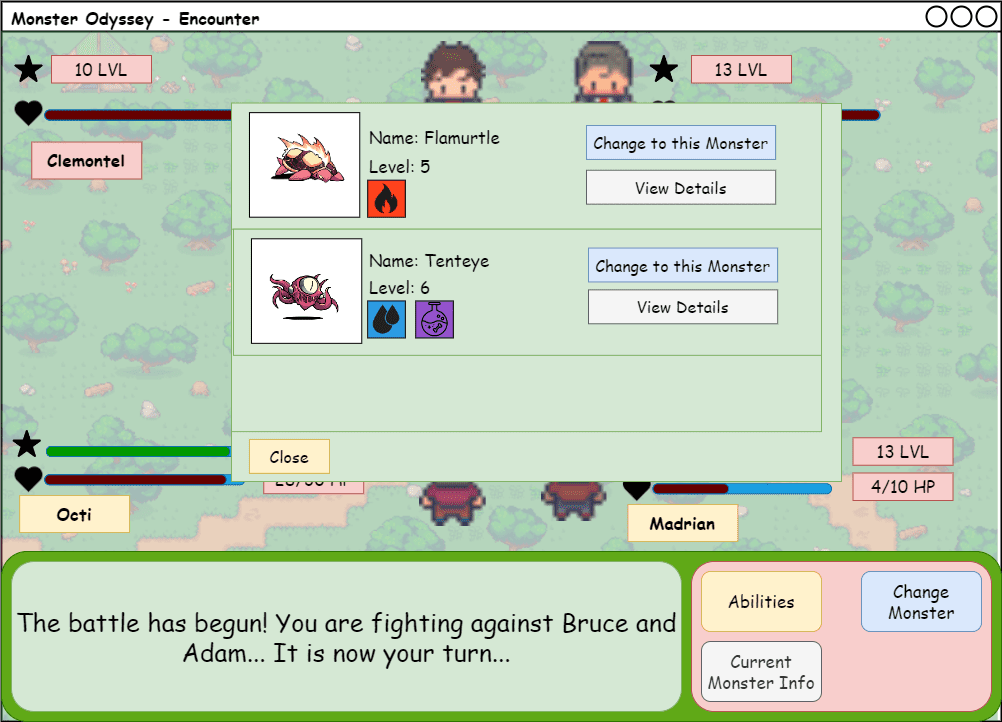
\includegraphics[width=\textwidth]{images/mockups/Encounter/Encounter2v2ChangeMonsterPopup.png}
        \caption{Mockup: \phantom{wechseln}Monster auswechseln Popup}
        \label{fig: Mockup: Monster auswechseln Popup}
    \end{subfigure}
    \hfill
    \begin{subfigure}[b]{0.4\textwidth}
        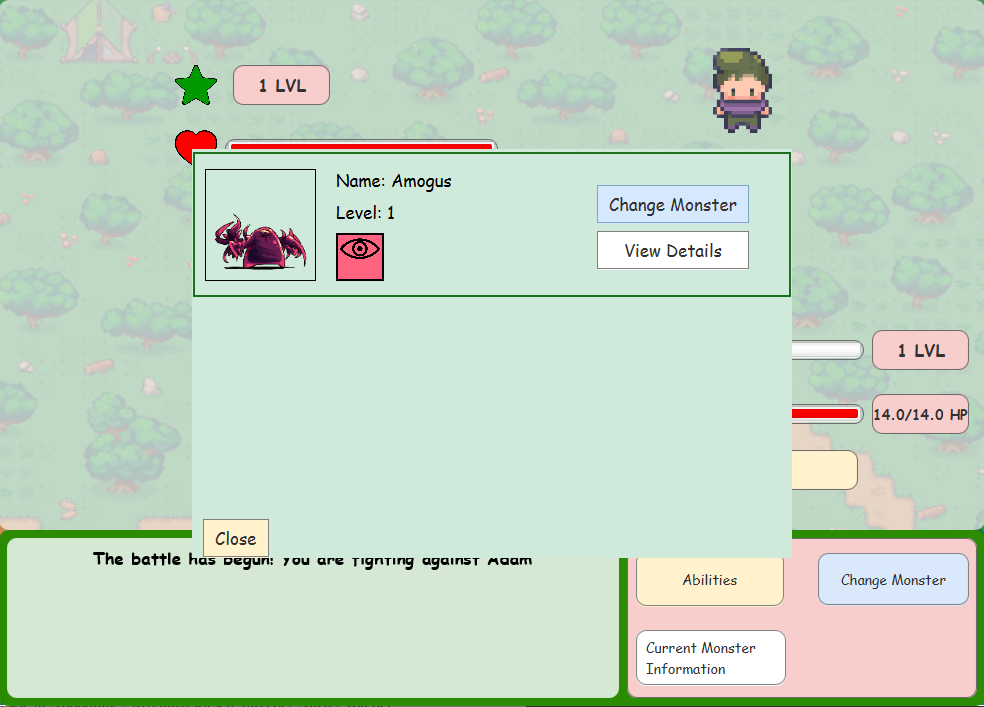
\includegraphics[width=\textwidth]{images/implementation/Encounter/monsterwechseln.PNG}
        \caption{Implementierung: Monster auswechseln Popup}
        \label{fig: Implementierung: Monster auswechseln Popup}
    \end{subfigure}
    \caption{Vergleich: Monster auswechseln Popup}
    \label{fig: Vergleich: Monster auswechseln Popup}
\end{figure}
\begin{figure}[H]
    \centering
    \begin{subfigure}[b]{0.4\textwidth}
        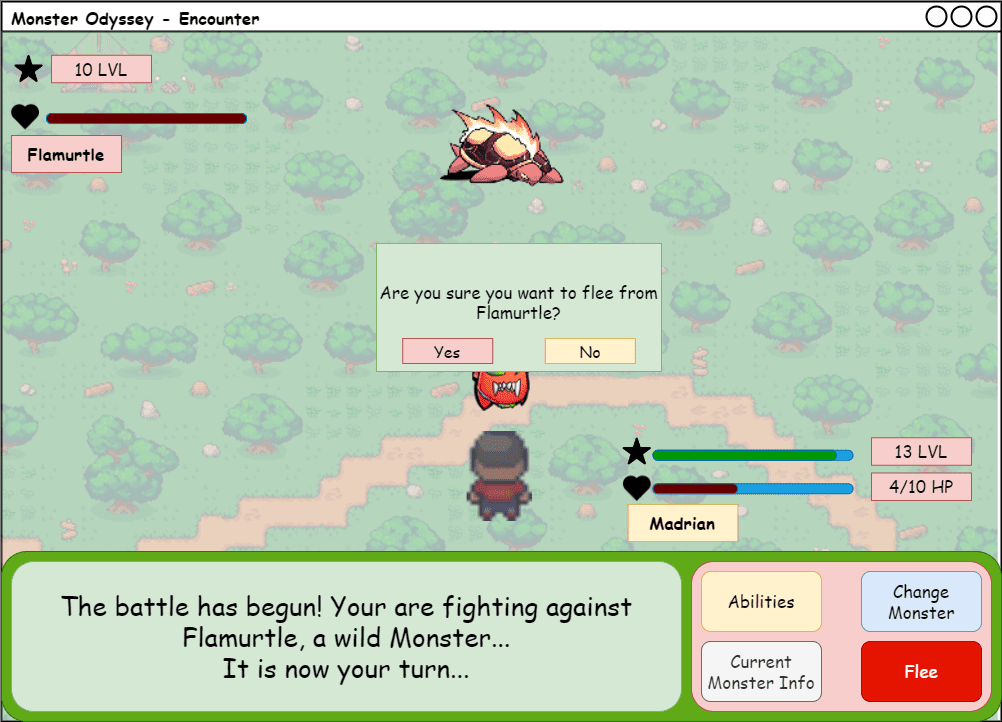
\includegraphics[width=\textwidth]{images/mockups/Encounter/EncounterWildFleePopUp.png}
        \caption{Mockup: \phantom{beimFlie}Popup beim Fliehen}
        \label{fig: Mockup: Popup beim Fliehen}
    \end{subfigure}
    \hfill
    \begin{subfigure}[b]{0.4\textwidth}
        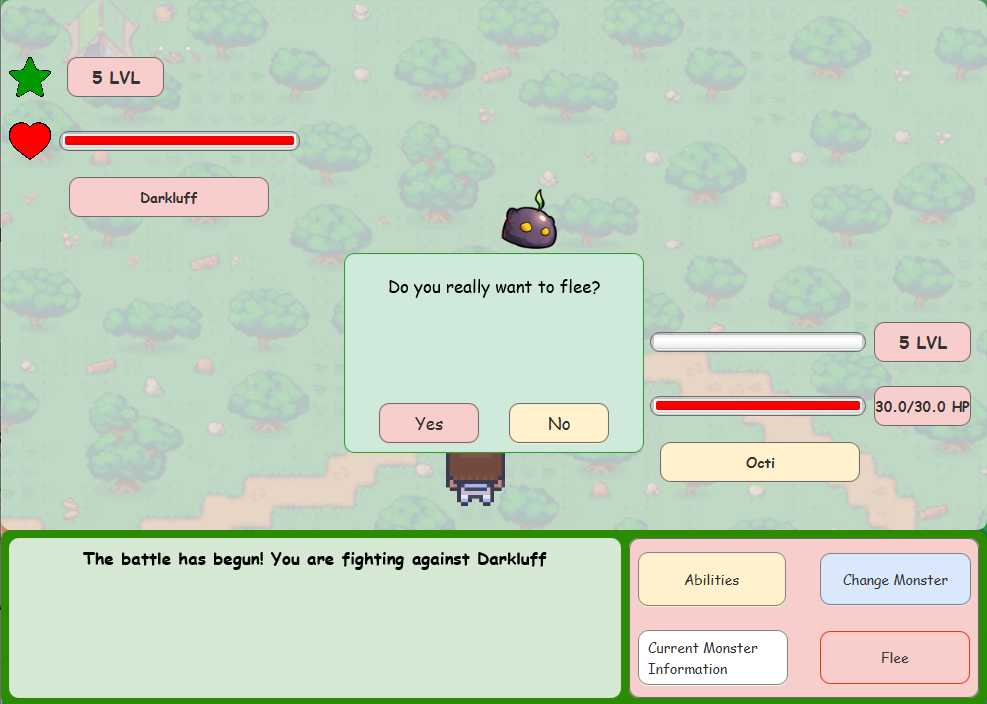
\includegraphics[width=\textwidth]{images/implementation/Encounter/fliehenpopup.PNG}
        \caption{Implementierung: Popup beim Fliehen}
        \label{fig: Implementierung: Popup beim Fliehen}
    \end{subfigure}
    \caption{Vergleich: Popup beim Fliehen}
    \label{fig: Vergleich: Popup beim Fliehen}
\end{figure}
\begin{figure}[H]
    \centering
    \begin{subfigure}[b]{0.4\textwidth}
        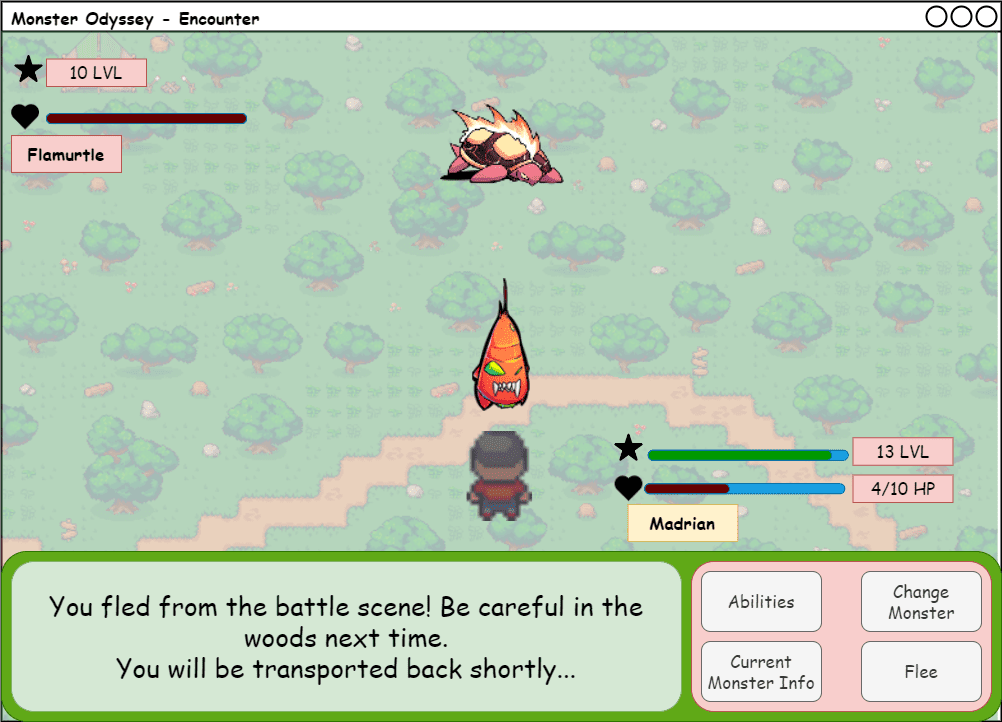
\includegraphics[width=\textwidth]{images/mockups/Encounter/EncounterWildFleed.png}
        \caption{Mockup: \phantom{desdes jetz}Von wildem Monster geflohen}
        \label{fig: Mockup: Von wildem Monster geflohen}
    \end{subfigure}
    \hfill
    \begin{subfigure}[b]{0.4\textwidth}
        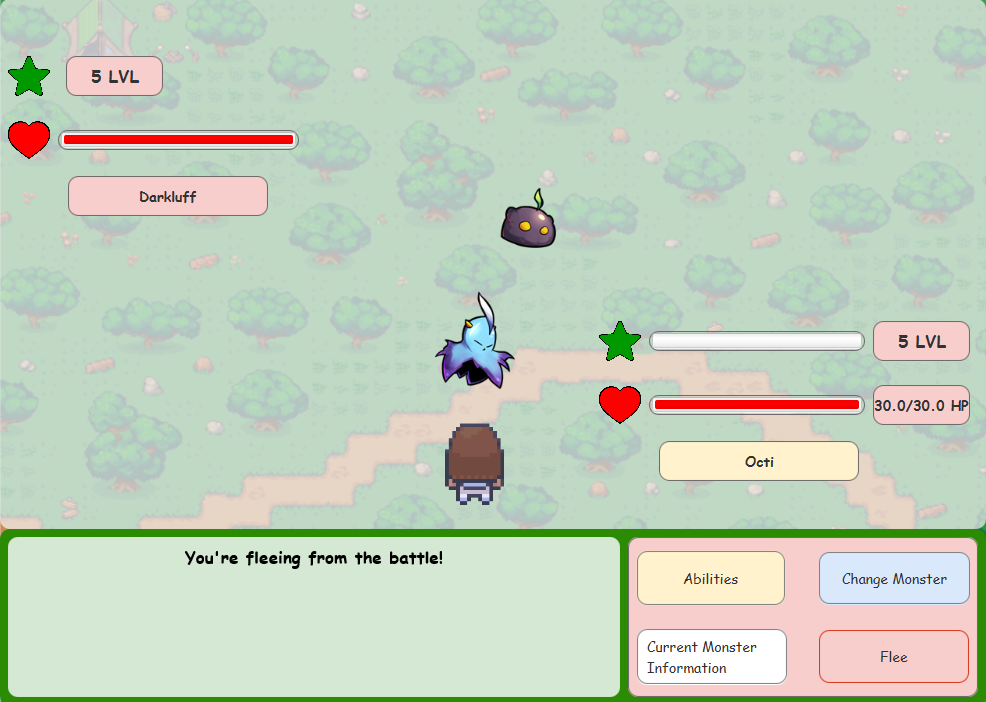
\includegraphics[width=\textwidth]{images/implementation/Encounter/vomkampfgeflohen.PNG}
        \caption{Implementierung: Von wildem Monster geflohen}
        \label{fig: Implementierung: Von wildem Monster geflohen}
    \end{subfigure}
    \caption{Vergleich: Von wildem Monster geflohen}
    \label{fig: Vergleich: Von wildem Monster geflohen}
\end{figure}